\setcounter{step}{0}
%------------------------------------------
% information doc
\subsection{Lasagne s brokolicou}
%------------------------------------------

\begin{ingredient}
%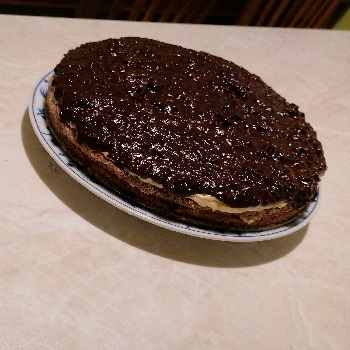
\includegraphics[height=5.5cm]{images/daim}
\def\portions{4}%
\textbf{{\normalsize Ingrediencie (\portions porcie):}}
%\vspace{0.5cm}
\begin{main}
	\item lasagnové pláty
	\item brokolica
	\item tvrdý syr
\end{main}
\begin{subingredient}{Bešamel}
	\item 50g maslo
	\item štipka soli
	\item 100g hladkej múky
	\item 500ml mlieka
	\item nejaké korenie
\end{subingredient}
\end{ingredient}
\begin{recipe}
\textbf{{\normalsize Príprava:}}
\begin{enumerate}

\item{Uvaríme brokolicu}
\item{Pripravíme si bešamel:}
\begin{enumerate}
\item{Roztopiť maslo, pridať múku}
\item{Pridávať mlieko}
\item{Osoliť, okoreniť}
\end{enumerate}

\item{Dáme do taniera vriacu vodu, postupne do nej namáčame pláty a ukladáme do zapekacej misy}
\item{Na vrstvu plátov dáme vrstvu bešamelu a brokolice (poprípade šunky)}
\item{Na poslednú vrstvu nedávame brokolicu, ale poukladáme/postrúhame tvrdý syr}
\item{Pečieme 30 minút na 180°}

\end{enumerate}
\end{recipe}

\begin{notes}

\end{notes}
\clearpage	